\documentclass{article}
\usepackage{amsmath}
\usepackage{amsfonts}
\usepackage{amssymb}
\usepackage[nomessages]{fp}
\usepackage{booktabs}
\usepackage{tikz,pgfplots}
\usepackage{enumerate}

\newcommand{\parcial}{\ensuremath{\dfrac{\partial}{\partial x}}}
\newcommand{\trad}[3]{#1 $\Rightarrow$ #2$\Rightarrow$ #3\\}
\newcommand{\derivada}[1]{\ensuremath{\dfrac{d}{dx} #1}}
\newcommand{\partes}[2]{\ensuremath{\int (#1)( \derivada{#2}) = (#1)(#2)- \int (#2) (\derivada{#1})}}

\newcommand{\sumar}[2]{
\FPeval{\resultado}{clip(#1+#2)}
\FPround \redondeado \resultado 2
\redondeado}

\newcommand{\restar}[2]{
\FPeval{\resultado}{clip(#1-#2)}
\FPround \redondeado \resultado 2
\redondeado}

\newcommand{\multiplicar}[2]{
\FPeval{\resultado}{clip(#1*#2)}
\FPround \redondeado \resultado 2
\redondeado}

\newcommand{\multitres}[3]{
\FPeval{\resultado}{clip(#1*#2*#3)}
\FPround \redondeado \resultado 2
\redondeado}

\newcommand{\dividir}[2]{
\FPeval{\resultado}{clip(#1/#2)}
\FPround \redondeado \resultado 2
\redondeado}

\newcommand{\elevar}[2]{
\FPeval{\resultado}{clip(#1^#2)}
\FPround \redondeado \resultado 2
\redondeado}

\newcommand{\cuadrado}[1]{\elevar{#1}{2}}
\newcommand{\productoi}[2]{\multitres{4}{#1}{#2}}
\newcommand{\DET}[3]{\restar{\cuadrado{#1}}{\productoi{#2}{#3}}}


\newcommand{\cuadratica}[3]{$#1x^2+(#2)x+(#3)=0$ \\
\begin{align*}
x&=\dfrac{-(#2)\pm \sqrt{(#2)^2-4(#1)(#3)}}{2(#1)}\\
\end{align*}
}
\newcommand{\resolvercuadratica}[3]{La soluci\'on a la ecuaci\'on $#1x^2+(#2)x+(#3)=0$ es
\begin{align*}
x&=\dfrac{-(#2)\pm \sqrt{(#2)^2-4(#1)(#3)}}{2(#1)}\\
&=\dfrac{-(#2)\pm \sqrt{\elevar{#2}{2}-4(\multiplicar{#1}{#3})}}{\multiplicar{2}{#1}}\\
&=\dfrac{-(#2)\pm \sqrt{\elevar{#2}{2}-\multitres{4}{#1}{#3}}}{\multiplicar{2}{#1}}\\
\end{align*}
}
\newcommand{\sumatoria}[3]{\ensuremath{\sum^{#1}_{#2} #3}}
\renewcommand{\cuadratica}[3]{
\begin{align*}
&#1x^2+(#2)x+(#3)=0\\
x&=\dfrac{-(#2)\pm \sqrt{(#2)^2-4(#1)(#3)}}{2(#1)}\\
\end{align*}
Como se puede ver, las ecuaciones cuadraticas pueden tener cero, una o dos soluciones reales dependiendo del valor de $(#2)^2-4(#1)(#3)$
}
\title{Funciones Cuadraticas \\\small{Matem\'aticas 10mo}\\\small{ColombiaCrece}}
\author{Sebasti\'an Rosales \\(3123211487, s.rosales2812@uniandes.edu.co)}


\begin{document}
\maketitle
\section{Explicaci\'on}
Ya hemos trabajado con las funciones lineales. Estas ten\'ian la forma:
\[y=mx+b\]
Donde m era la pendiente de la gr\'afica y b era el corte con el eje Y. 
Vamos a empezar a trabajar con un nuevo tipo de funci\'on, las funciones cuadr\'aticas. Estas funciones tienen la forma

\textbf{\[y(x)=ax^{2}+bx+c\]}
La forma de estas funciones es: \\
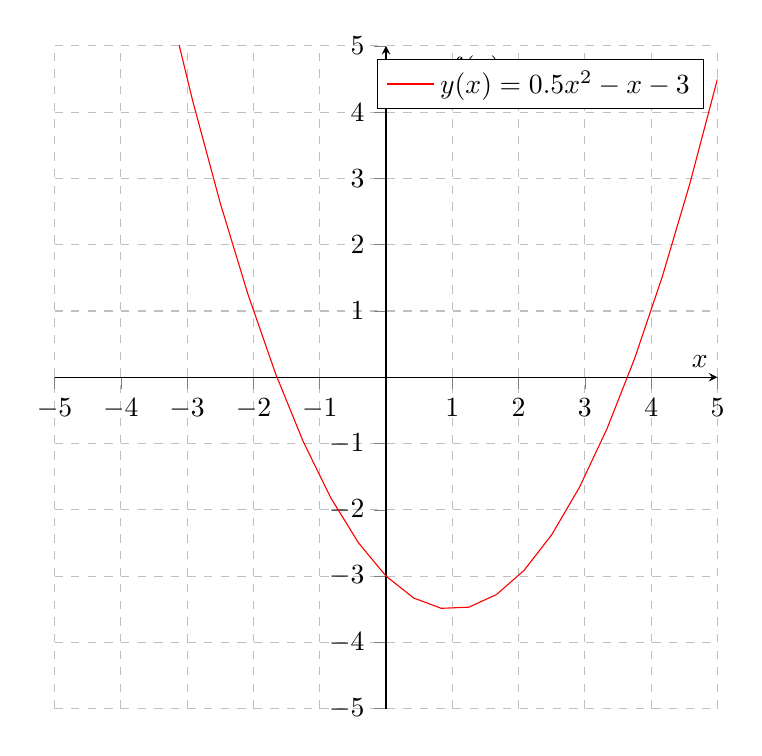
\begin{tikzpicture}
\begin{axis}[axis x line=center, axis y line=center,,xtick={-5,-4,...,5},ytick={-5,-4,...,5},width=10cm, height=10cm,xlabel={$x$}, ylabel={$y=f(x)$},tick align=outside,xmin=-5,xmax=5, ymin=-5,ymax=5,xmajorgrids,ymajorgrids,grid style={dashed, gray!50}]
\addplot [no marks,red]{0.5*x^2-x-3};
\addlegendentry{$y(x)=0.5x^2-x-3$};
\end{axis}
\end{tikzpicture}\\




As\'i como en la funci\'on lineal identificar la pendiente y el corte con el eje era importante, ac\'a, en las funciones cuadr\'aticas tambi\'en tenemos que aprender a identificar las partes de la funci\'on. Revisemos cuales son las partes de la funci\'on $y(x)=3x^2-4x+5$ 
\begin{description}
\item[a] Es el factor que acompa\~na al \'unico  t\'ermino cuadr\'atico(ojo con el signo):\\ $y(x)=\underbrace{+3}_a x^{2}-4x+5$.
\item[b] Es el factor que acompa\~na al \'unico  t\'ermino lineal(ojo con el signo): \\$y(x)=3x^{2}\underbrace{-4}_bx+5$.
\item[c] Es el \'unico t\'ermino que esta solo(ojo con el signo): \\$y(x)=3x^{2}-4x\underbrace{+5}_c$.
\end{description}

Ya sabemos identificar las partes de una funci\'on cuadratica. Practiquemos : 
\begin{align}
y(x)&=3x^2+6x+3\\
w(x)&=x^2-4x+4\\
z(x)&=2x^2-6x\\
f(x)&=30-2x^2-4x\\
g(x)&=2x^2-x^2-3x+2\\
h(x)&=5x+2x^3-20-x^2+6\\
k(x)&=10-3x^2+6x+2x^2-15-2x
\end{align}
\begin{center}
\begin{tabular}{|c|p{2cm}|p{2cm}|p{2cm}|}
 \hline
F(x)&a&b&c\\
\hline
y&&&\\
w&&&\\
z&&&\\
f&&&\\
g&&&\\
h&&&\\
k&&&\\
\hline
\end{tabular}
\end{center}
Si dese\'aramos comparar la ecuaci\'on de las funci\'ones cuadr\'aticas con la de  las funciones lineales, tendriamos los siguiente: 
\[\begin{matrix}
y(x)&=&ax^{2}+&bx&+c\\
y(x)&=&&mx&+b\\
\end{matrix}\]


Ac\'a podemos notar que las ecuaciones cuadr\'aticas son ecuaciones lineales m\'as un termino con $x^{2}$ y que la labor que cumpl\'ia b en las lineales, la cumple c en la cuadr\'aticas. Veamos que hacen los n\'umeros a y c en las funciones cuadr\'aticas:\\
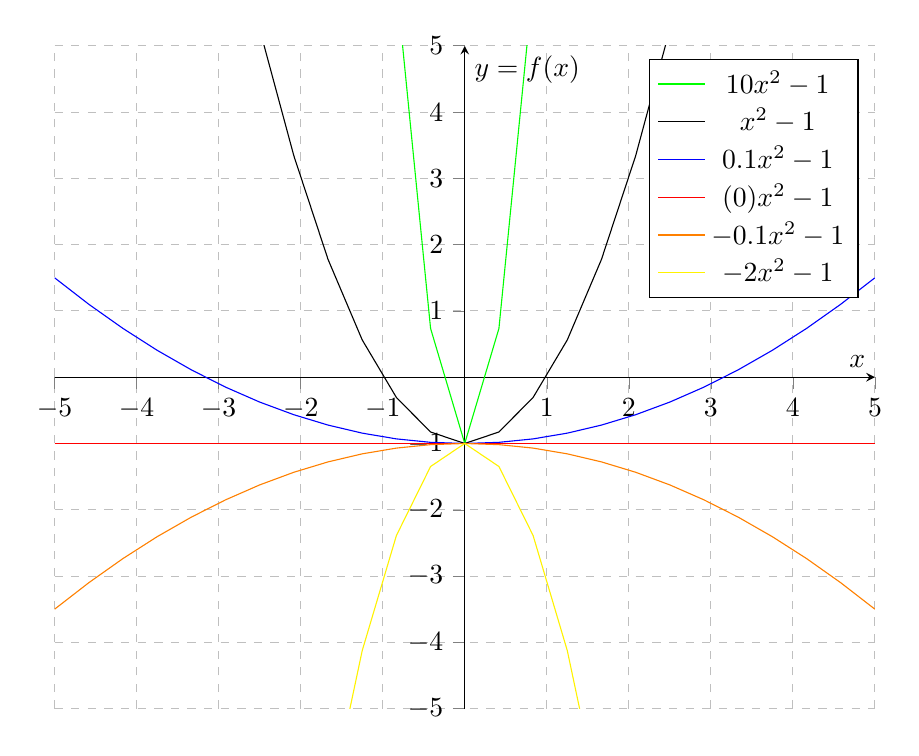
\begin{tikzpicture}
\begin{axis}[axis x line=center, axis y line=center,,xtick={-5,-4,...,5},ytick={-5,-4,...,5},width=12cm, height=10cm,xlabel={$x$}, ylabel={$y=f(x)$},tick align=outside,xmin=-5,xmax=5, ymin=-5,ymax=5,xmajorgrids,ymajorgrids,grid style={dashed, gray!50}]
\addplot [no marks,green]{10*x^2-1};
\addlegendentry{$10x^2-1$};
\addplot [no marks,black]{x^2-1};
\addlegendentry{$x^2-1$};
\addplot [no marks,blue]{0.1*x^2-1};
\addlegendentry{$0.1x^2-1$};
\addplot [no marks,red]{-1};
\addlegendentry{$(0)x^2-1$};
\addplot [no marks,orange]{-0.1*x^2-1};
\addlegendentry{$-0.1x^2-1$};
\addplot [no marks,yellow]{-2*x^2-1};
\addlegendentry{$-2x^2-1$};
\end{axis}
\end{tikzpicture}

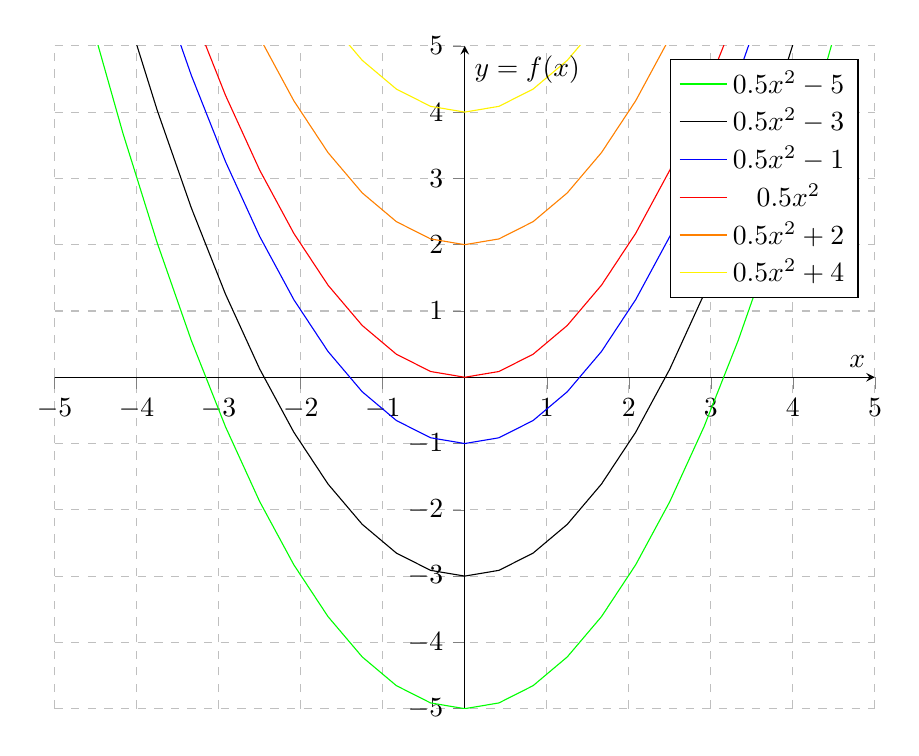
\begin{tikzpicture}
\begin{axis}[axis x line=center, axis y line=center,,xtick={-5,-4,...,5},ytick={-5,-4,...,5},width=12cm, height=10cm,xlabel={$x$}, ylabel={$y=f(x)$},tick align=outside,xmin=-5,xmax=5, ymin=-5,ymax=5,xmajorgrids,ymajorgrids,grid style={dashed, gray!50}]
\addplot [no marks,green]{0.5*x^2-5};
\addlegendentry{$0.5x^2-5$};
\addplot [no marks,black]{0.5*x^2-3};
\addlegendentry{$0.5x^2-3$};
\addplot [no marks,blue]{0.5*x^2-1};
\addlegendentry{$0.5x^2-1$};
\addplot [no marks,red]{0.5*x^2};
\addlegendentry{$0.5x^2$};
\addplot [no marks,orange]{0.5*x^2+2};
\addlegendentry{$0.5x^2+2$};
\addplot [no marks,yellow]{0.5*x^2+4};
\addlegendentry{$0.5x^2+4$};
\end{axis}
\end{tikzpicture}\\


Existe un caso particular que es de nuestros interes y es  cuando y=0 por que representa las \textbf{raices de la ecuaci\'on cuadratica} y este caso se soluciona asi: \\
\cuadratica{a}{b}{c}
\newline
Veamos un par de ejemplos: 
\resolvercuadratica {1}{5}{4}
\begin{align*}
x&=\dfrac{-5\pm 4}{2}\\
x_1&=\dfrac{-5+4}{2}=-0.5\\
x_2&=\dfrac{-5-4}{2}=-4.5\\
\end{align*}
\resolvercuadratica {2}{4}{2}
\begin{align*}
x&=\dfrac{-4\pm 0}{4}\\
x_1&=\dfrac{-4}{4}=1\\
x_2&=\dfrac{-4}{4}=1\\
\end{align*}
\section{Taller}
En este taller vamos a trabajar primero desde una gr\'afica hacia una ecuación, y luego desde una ecuación hacia una gr\'afica. \\
Veamos las siguientes gr\'aficas:  \\
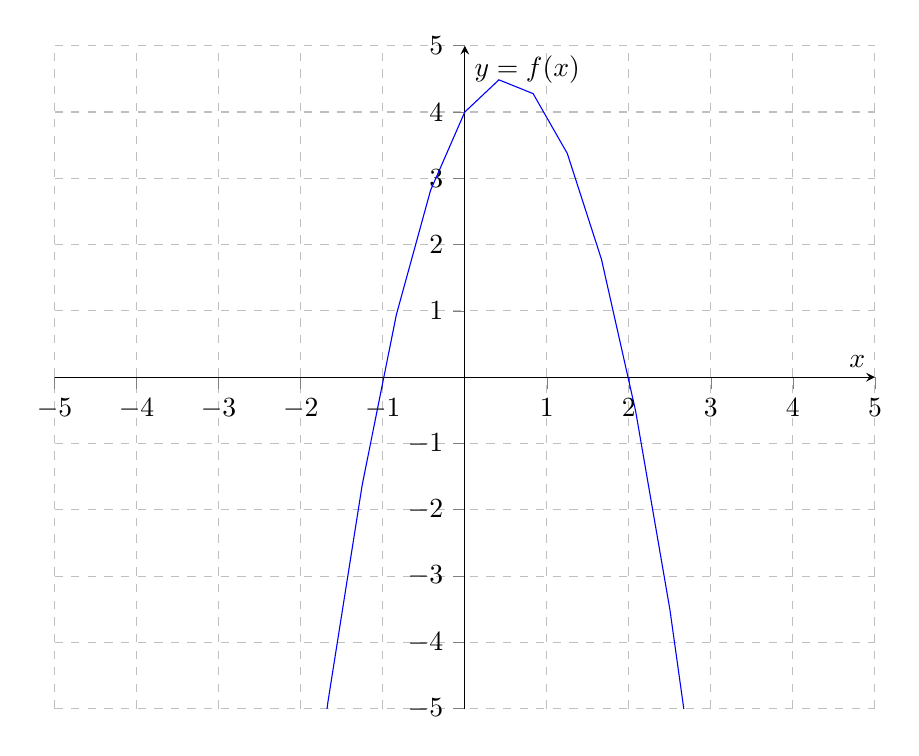
\begin{tikzpicture}
\begin{axis}
[axis x line=center, axis y line=center,,xtick={-5,-4,...,5},ytick={-5,-4,...,5},width=12cm, height=10cm,xlabel={$x$}, ylabel={$y=f(x)$},tick align=outside,xmin=-5,xmax=5, ymin=-5, ymax=5, xmajorgrids, ymajorgrids, grid style={dashed, gray!50}]
\addplot [no marks,blue]{-2*x^2+2*x+4};
\end{axis}
\end{tikzpicture}
\\Responde la siguientes preguntas:\\
\begin{enumerate}
\item ?`$ a$ es positivo o negativo?
\item ?`Cu\'anto vale $ c$ ? 
\item  Teniendo en cuenta los dos resultados anteriores, ?` Cu\'al de las siguientes crees que es la funci\'on que describe la gr\'afica?
\begin{enumerate}[a)]
\item $f(x)=2x^2+2x$
\item  $f(x)=-2x^2+2x$
\item  $f(x)=2x^2+2x+4$
\item  $f(x)=-2x^2+2x-4$
\item  $f(x)=2x^2+2x-4$
\item  $f(x)=-2x^2+2x+4$
\end{enumerate}
\item ?`Cuanto valen las raices de esta ecuaci\'on? 
\end{enumerate}
\newpage
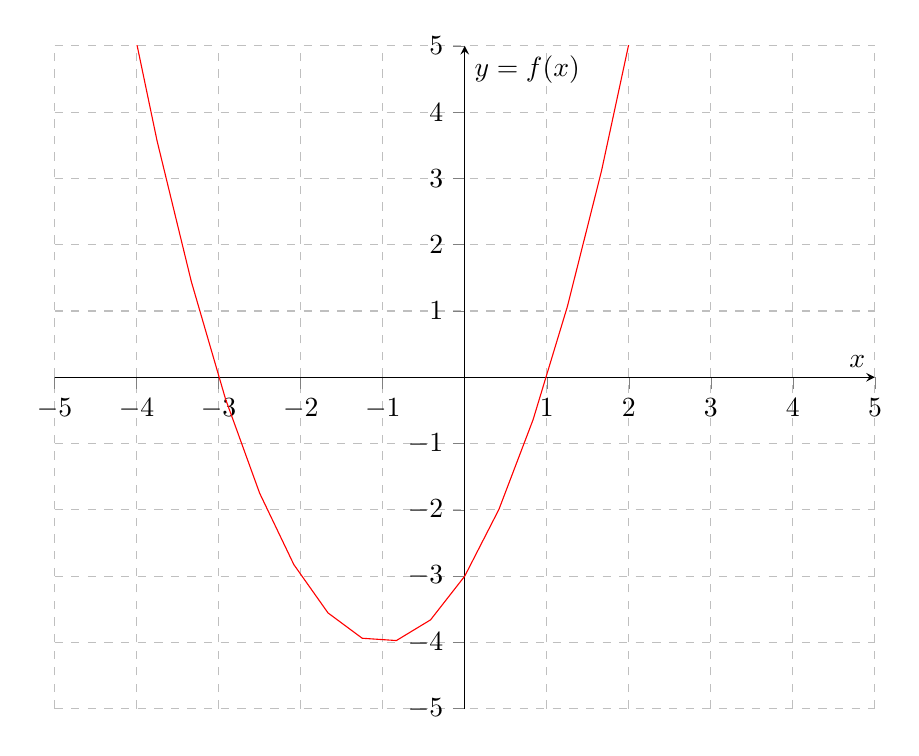
\begin{tikzpicture}
\begin{axis}
[axis x line=center, axis y line=center,,xtick={-5,-4,...,5},ytick={-5,-4,...,5},width=12cm, height=10cm,xlabel={$x$}, ylabel={$y=f(x)$},tick align=outside,xmin=-5,xmax=5, ymin=-5, ymax=5, xmajorgrids, ymajorgrids, grid style={dashed, gray!50}]
\addplot [no marks,red]{x^2+2*x-3};
\end{axis}
\end{tikzpicture}
\\Responde la siguientes preguntas:\\
\begin{enumerate}
\item ?`$ a$ es positivo o negativo?
\item ?`Cu\'anto vale $ c$ ? 
\item  Teniendo en cuenta los dos resultados anteriores, ?` Cu\'al de las siguientes crees que es la funci\'on que describe la gr\'afica?
\begin{enumerate}[a)]
\item $f(x)=x^2+2x$
\item  $f(x)=-x^2+2x$
\item  $f(x)=x^2+2x+3$
\item  $f(x)=x^2+2x-3$
\item  $f(x)=-x^2+2x-3$
\item  $f(x)=--x^2+2x+3$
\end{enumerate}
\item ?`Cuanto valen las raices de esta ecuaci\'on? 
\end{enumerate}
\newpage
Ahora, vamos a analizar esta funci\'on
\begin{equation}
f(x)=x^2-3x-4
\end{equation}
Responde la siguientes preguntas:\\
\begin{enumerate}
\item ?`Cuanto vale $a$, $b$, $c$?
\item ?`Cuanto valen las raices? 
\item  Teniendo en cuenta los dos resultados anteriores dibuja la gr\'afica de esa funci\'on. \\
\begin{tikzpicture}
\begin{axis}
[axis x line=center, axis y line=center,,xtick={-5,-4,...,5},ytick={-5,-4,...,5},width=12cm, height=10cm,xlabel={$x$}, ylabel={$y=f(x)$},tick align=outside,xmin=-5,xmax=5, ymin=-5, ymax=5, xmajorgrids, ymajorgrids, grid style={dashed, gray!50}]
\end{axis}
\end{tikzpicture}
\end{enumerate}
\newpage
\section{Tarea}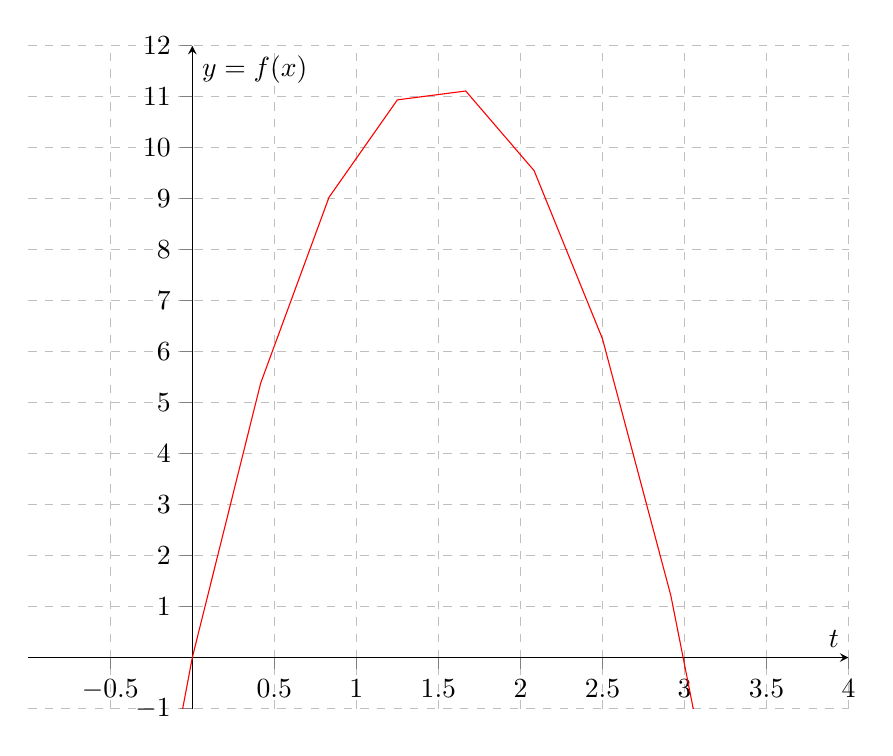
\begin{tikzpicture}
\begin{axis}
[axis x line=center, axis y line=center,,xtick={-0.5,0,...,4},ytick={-1,0,...,12},width=12cm, height=10cm,xlabel={$t$}, ylabel={$y=f(x)$},tick align=outside,xmin=-1,xmax=4, ymin=-1, ymax=12, xmajorgrids, ymajorgrids, grid style={dashed, gray!50}]
\addplot [no marks,red]{-5*x^2+15*x};
\end{axis}
\end{tikzpicture}
 La anterior es la gr\'afica  funci\'on de la altura contra el tiempo  de un proyectil en movimiento parab\'olic0 descrita por: $y(t)= \frac{1}{2}gt^2+v_0t + y_0$\\
\begin{enumerate}
\item ?`$ a$ es positivo o negativo?
\item ?`Cu\'anto vale $ c$ ? 
\item  Teniendo en cuenta los dos resultados anteriores, ?` Cu\'al de las siguientes crees que es la funci\'on que describe la gr\'afica?
\begin{enumerate}[a)]
\item $f(x)=-5x^2+15x$
\item  $f(x)=5x^2+15x$
\item  $f(x)=-5x^2+15x+3$
\item  $f(x)=5x^2+15x-3$
\end{enumerate}
\item Teniendo en cuenta el resultado anterior y que la ecuaci\'on que describe el moviemiento parab\'olico ?`Cu\'anto vale $g$ y $v_0$?
\item ?`Cuanto valen las raices de esta ecuaci\'on? `?Qu\'e significan f\'isicamente?

\end{enumerate}
\newpage
Ahora, vamos a analizar esta funci\'on
\begin{equation}
f(x)=x^2+4x+4
\end{equation}
Responde la siguientes preguntas:\\
\begin{enumerate}
\item ?`Cuanto vale $a$, $b$, $c$?
\item ?`Cuanto valen las raices? 
\item  Teniendo en cuenta los dos resultados anteriores dibuja la gr\'afica de esa funci\'on. \\
\begin{tikzpicture}
\begin{axis}
[axis x line=center, axis y line=center,,xtick={-5,-4,...,5},ytick={-5,-4,...,5},width=12cm, height=10cm,xlabel={$x$}, ylabel={$y=f(x)$},tick align=outside,xmin=-5,xmax=5, ymin=-5, ymax=5, xmajorgrids, ymajorgrids, grid style={dashed, gray!50}]
\end{axis}
\end{tikzpicture}
\end{enumerate}
\end{document}